\chapter{Case Study}
\label{chapter:case_study}
After completing the theoretical part by explaining when and how to combine languages or separate them, this section deals with the methodology of how to identify each modeling language and how to apply the indicators in a practical environment in general.

\section{Methodology}

%------------------------------------------------------------------------------
\begin{wraptable}{r}{0.5\textwidth}
\begin{tabular}{@{}ll@{}}
\toprule
Categories                   & Weighting \\ \midrule
Documentation style          & 1         \\
Preceding process map       & 1         \\
Characteristics of work      & 2         \\
Characteristics of process   & 2         \\
Characteristics of decisions & 2         \\
Control flow                 & 1         \\
Intervention at run-time     & 1         \\
Objective                    & 2         \\
Type of process              & 2         \\
Typical application          & 1         \\ \bottomrule
\end{tabular}
\caption{Each category is assigned a specific weight to calculate the match's percentage.}
\label{tab:indicator_weight}
\end{wraptable}
%-------------------------------------------------------------------------------------
In Chapter \ref{chapter:indicators}, the Categories stated in Table \ref{tab:indicator_weight} were presented along with corresponding terms and definitions. To apply them and calculate the matching language, each category is assigned a weight. As seen in the mentioned table, some categories are weighted with factor one, some are weighted with two. This depends on which indicator is more important than the other ones. The characteristics of a process or work are more important than e.g. the typical application. The two-point indicators describe the main characteristics of a process and should result from process discovery, making it clear which language to use mainly. These indicators are supported by the one-point ones, which describe more generally how documentation and surrounding work looks like. Basically, the two-point indicators are the core-indicators and the single-point indicators are the supporting ones. \\
The next step is to build a decision logic that implements the indicators, their weight and generate an output value. \\
Looking at the requirements of this process indicates that DMN is the suitable language therefore. The documentation is a spreadsheet with all values, followed by a decision tree on how to calculate the corresponding points. Overall, this is a data-centric process incorporating calculations and data handling. Furthermore, there is no control flow required but dependencies are necessary to provide a recommendation based on the matching points. The fit for DMN is, according to the indicators, 100 percent. \\

\begin{figure}
\centering
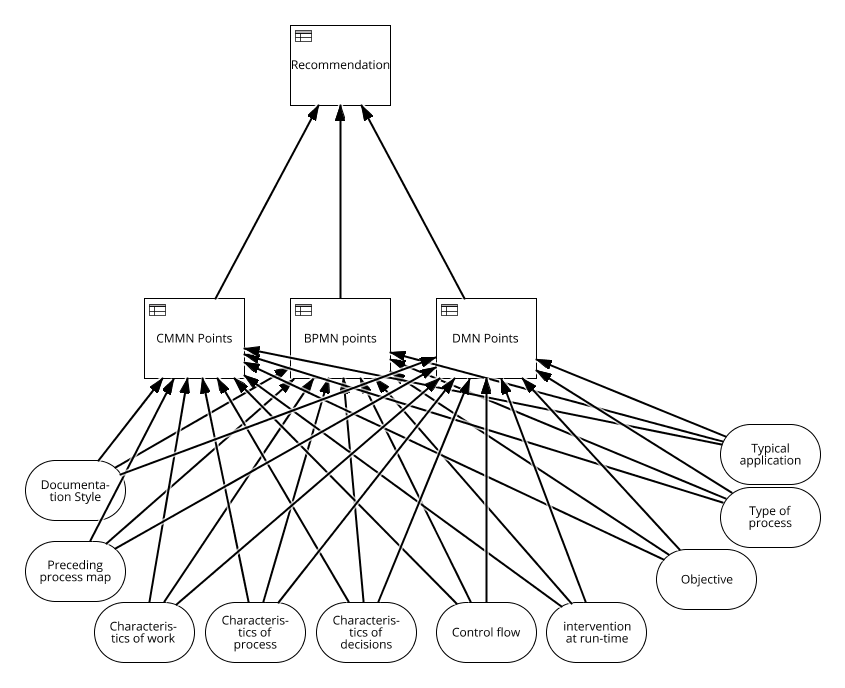
\includegraphics[width=0.9\textwidth]{../figures/chapter_casestudy/Recommendation_engine.png} 
\caption{The recommendation engine denoted as a DRG.}
\label{fig:recommendation_engine}
\end{figure}

An overview of the decision logic and the \ac{DRG} provides Figure \ref{fig:recommendation_engine}. Here we can see three levels of decision-making: The lower level is comprised of all the input data elements that contain the indicator categories and the corresponding terms. Located one level above are three decision-logic elements containing the decision logic to calculate the matching points according to each set of indicators. As stated in Chapter \ref{chapter:indicators}, the indicator itself is a set of terms. Each decision at this level incorporates this aggregation and sums up how many points match.\newpage To assure that all tables have the same input data and the matching is unique, each input data element is connected to all the summarizing tables. If, for instance, a modeler enters \textit{Flowchart} in the \textit{Preceding Process map} element, the BPMN table is triggered, whereas the remaining tables are not. \\
The highest level comprises the recommendation decision. The amount of points is passed to this decision element, whose output is the recommended language. Here, a certain threshold is set to achieve a distinct recommendation of one suitable language, instead of suggesting a combined approach. The main thought behind this threshold was to create models according to the \textit{separation of concerns} paradigm mentioned in Chapter \ref{chapter:combination}. In this case, the threshold is set to an 80-percent-matching. Every match below this threshold is recommended to iterate once again through process discovery and refine the output. Consequently, each recommendation is intended to result in a process that features high cohesion and low coupling, similar to software engineering. \\
In a last step, the models should be aggregated in a larger macro model that shows how the different processes work together and serves as an orchestration for the whole process. All the sub-processes will be handled by this macro process guiding either a workflow or a case to the desired output. Here we can see that DMN will never serve as a macro-process due to the complementary aspect and the lack of interfaces to different modeling languages. Contrary to the specification \cite{DMNspec2016}, DMN is only suitable for very few use cases to serve as a standalone model. These few use cases are mainly decisions and data handling in combined approaches. \\
In the next sections, we will analyze the output of process discovery done by the eKultur GmbH and check the results with the indicators. Furthermore, the indicators state if the process discovery is sufficient or another iteration is necessary. Afterwards, the decision logic recommends the suitable modeling language, which is then applied to the process discovery results. The last step is to create the models and combine them according to the findings in Chapter \ref{chapter:combination}.

\section{Company audit process}
In this section, a key process taken from the eKultur GmbH process discovery will be examined. Before the examination commences in the following subsections, a brief overview of the process landscapes and the context of the processes is helpful to understand the big picture. \\
The eKultur project's objective is to level up the touring theater production industry to a digital industry instead of a pen on paper one as it currently is.\newpage The first objective and simultaneously the first milestone is to offer a platform where each participant - may it be directors, mechanics, suppliers or actors - is able to register and upload information about the person itself and the corresponding company. Eventually, the industry will move from a personal address book storing the information on to the platform synchronizing it. \\
One of the platform's most essential parts is to ascertain the authenticity of each member and each company, since the companies are intended to conclude contracts such as hiring actors, renting stages or selling theater productions to municipalities. For this purpose, the \textit{Company audit} process was discovered.

\subsection{Sub-processes}
In Appendix A, the process discovery documentation is provided which can is summarized under \ref{fig:company_audit_PM}. The process map shows seven distinct steps to take which have not beend organized in any particular order. According to \cite{Verner2004}, the process discovery was done in a bottom-up way with a top-down view. First, the process map was created to organize the steps that are involved in \textit{Company audit} process, followed by an analysis of the sub-processes that are called to fulfill the checks.

%---------------------------------------------------------------
\begin{figure}
\centering
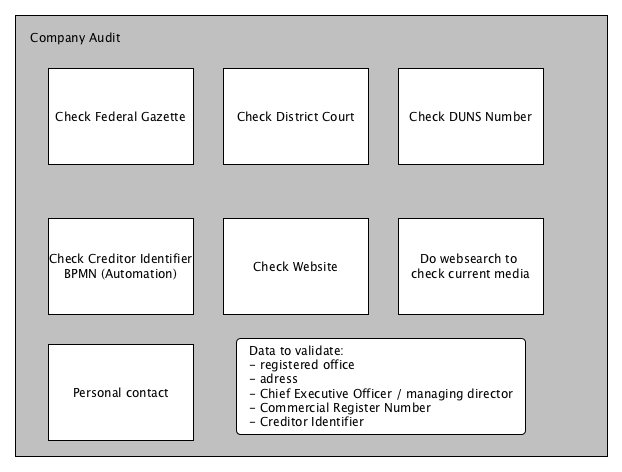
\includegraphics[width=0.9\textwidth]{../figures/chapter_casestudy/Company_audit_PM.png} 
\caption{Company Audit process map result from a first iteration of process discovery.}
\label{fig:company_audit_PM}
\end{figure}
%----------------------------------------------------------------

\subsubsection{Check Federal Gazette}
The objective of this process is to consult the federal commercial registry where companies obtain a commercial register number. This portal provides information about the current annual accounts and can be searched for keywords and companies. eKultur's auditor is intended, as the process discovery documentation states in Appendix A, to consult the Federal Gazette and to search for the company. Ideally, the auditor checks the latest annual accounts sheet and the date published. If the result confirms an active status, the auditor may set the internal status also to active and proceeds with the remaining checks. \\

% Please add the following required packages to your document preamble:
% \usepackage{graphicx}
\begin{table}[]
\centering
\resizebox{\textwidth}{!}{%
\begin{tabular}{lllll}
\hline
Categories                   & Check Federal Gazette matches       & BPMN Points & CMMN Points & DMN Points \\ \hline
Documentation style          & Directives                          & 1           & 0           & 0          \\
Preceding process map        & Cluster                             & 0           & 1           & 0          \\
Characteristics of work      & routine, predictable                & 2           & 0           & 0          \\
Characteristics of process   & rigid, predefined, workflow-centric & 2           & 0           & 0          \\
Characteristics of decisions & Simple (either / or)                & 2           & 0           & 0          \\
Control flow                 & Definite control flow, required     & 1           & 0           & 0          \\
Intervention at run-time     & No                                  & 1           & 0           & 0          \\
Objective                    & Automated workflow execution        & 2           & 0           & 0          \\
Type of process              & Business process                    & 2           & 0           & 0          \\
Typical application          & Accounting                          & 1           & 0           & 0          \\ \hline
\multicolumn{2}{l}{Percentage}                                     & 93,33       & 6,67        & 0          \\ \hline
\end{tabular}%
}
\caption{Indicator application on the \textit{Check Federal Gazette} process.}
\label{tab:federal_gazette}
\end{table}

Table \ref{tab:federal_gazette} shows the matches after applying the indicators on the process. As described by the process documentation, the main part of work is comprised of routine aspects such as consulting the Federal Gazette to check the annual accounts. The process neither requires any run-time intervention, nor can it be fully automated. On the other hand, it is predefined and predictable to a certain point: Either the status is \textit{active} or \textit{inactive} afterwards. Furthermore, a strict control flow is intended along with simple either / or decisions and the objective is to automate the workflow. The latter might not be completely achievable due to a missing API to the Federal Gazette's database. \enlargethispage{1\baselineskip}\\
The table's last row shows the percentage of the matches indicating that BPMN is the recommended modeling language and Figure \ref{fig:federal_gazette_BPMN} represents the corresponding model. 

\begin{sidewaysfigure}
\centering 
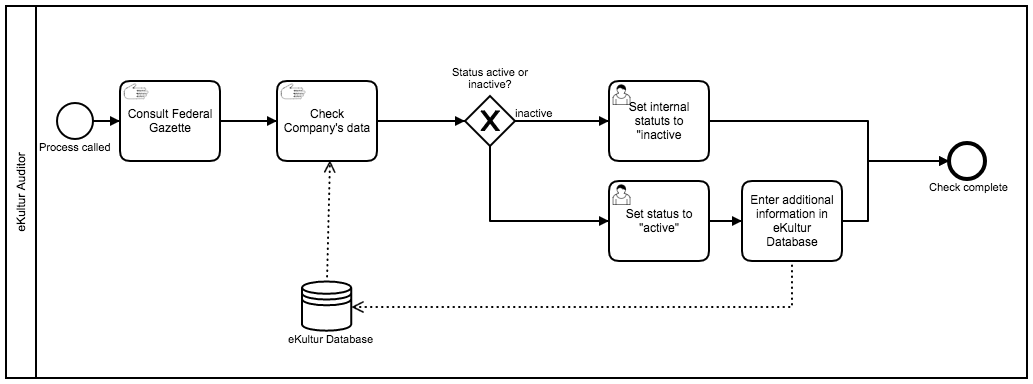
\includegraphics[scale=0.4]{../figures/chapter_casestudy/company_audit/BPMN_Check_Bundesanzeiger.png} 
\caption{\textit{Check Federal Gazette} process modeled in BPMN.}
\label{fig:federal_gazette_BPMN}
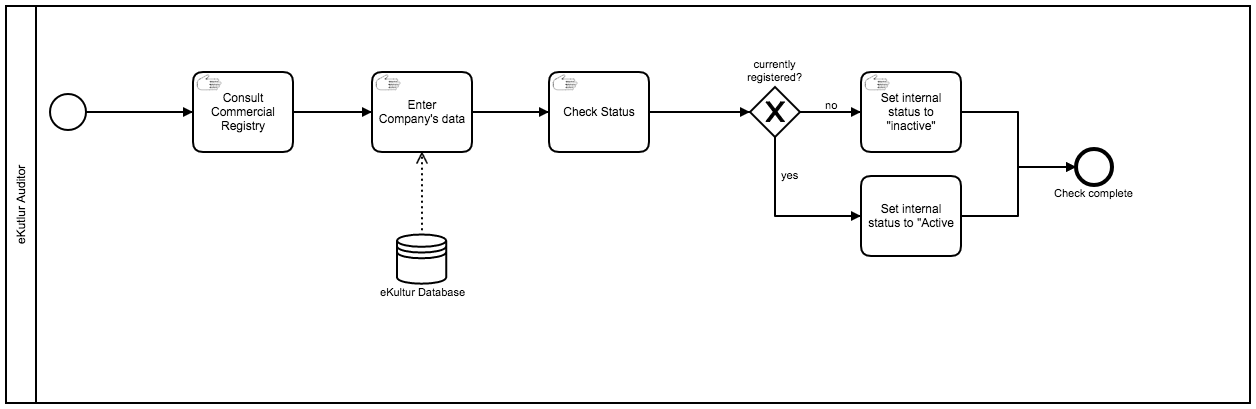
\includegraphics[scale=0.4]{../figures/chapter_casestudy/company_audit/BPMN_Check_Disctrict_Court.png} 
\caption{\textit{Check District Court} process modeled in BPMN.}
\label{fig:district_court_BPMN}
\end{sidewaysfigure}

\subsubsection{Check District Court}
\textit{Check District Court} is a rather small process that deals with identifying whether the local commercial registry lists the audited company as \textit{currently registered} or not. Different to the \textit{Check Federal Gazette} process, the auditor is not able to see the annual balance sheet but only a status and, if necessary, additional information about the company's commercial registration. \\
Similar to \textit{Check Federal Gazette}, the process comprises only routine elements without the necessity of run-time adapting or planning. Furthermore, a strict control flow is required and simple decisions are sufficient for this check. Conclusively, this process should be modeled in BPMN, which is emphasized by the indicators shown in Table \ref{tab:district_court} along with the resulting model in Figure \ref{fig:district_court_BPMN}. 

% Please add the following required packages to your document preamble:
% \usepackage{booktabs}
% \usepackage{graphicx}
\begin{table}[]
\centering
\resizebox{\textwidth}{!}{%
\begin{tabular}{@{}lllll@{}}
\toprule
Categories                   & Check District Court matches    & BPMN Points & CMMN Points & DMN Points \\ \midrule
Documentation style          & Directives                      & 1           & 0           & 0          \\
Preceding process map        & Cluster                         & 0           & 1           & 0          \\
Characteristics of work      & Routine                         & 2           & 0           & 0          \\
Characteristics of process   & Predefined, workflow-centric    & 2           & 0           & 0          \\
Characteristics of decisions & Simple (either / or)            & 2           & 0           & 0          \\
Control flow                 & Definite control flow, required & 1           & 0           & 0          \\
Intervention at run-time     & No                              & 1           & 0           & 0          \\
Objective                    & Automated workflow execution    & 2           & 0           & 0          \\
Type of process              & Business process                & 2           & 0           & 0          \\
Typical application          & Accounting                      & 1           & 0           & 0          \\ \midrule
\multicolumn{2}{l}{Percentage}                                 & 93,33       & 6,67        & 0          \\ \bottomrule
\end{tabular}%
}
\caption{Indicator application on the \textit{Check District Court} process.}
\label{tab:district_court}
\end{table}

\subsubsection{Check DUNS Number}
In the \textit{Check DUNS Number} process, the auditor is intended to consult the \ac{DUNS} and enter the company's information. \ac{DUNS} is a system that extracts information about companies and public institutions, among others, from the commercial registry and provides information about the management, activity, address and website. During a test of the system by eKultur GmbH it was noted, that some information provided by the DUNS has been deprecated. The process cannot be completely automated for two reasons: First, the system has no API to connect eKultur's database to perform automated checks. Second, in some cases the DUNS number must be obtained manually, whereas different companies already had one without registering. \\
As already noticed, the process comprises routine elements, is predefined as seen in the process documentation in Appendix A and the output is predictable. The process features a strict control flow and simple decisions without the necessity for run-time adjustment. Overall, the indicator table recommends BPMN for this process with manual tasks due to the lacking interface to the DUNS network. Table \ref{tab:check_DUNS} summarizes the matches and Figure \ref{fig:duns_number_BPMN} shows the process modeled in BPMN. 

% Please add the following required packages to your document preamble:
% \usepackage{graphicx}
\begin{table}[]
\centering
\resizebox{\textwidth}{!}{%
\begin{tabular}{lllll}
\hline
Categories                   & Check DUNS Number matches                       & BPMN Points & CMMN Points & DMN Points \\ \hline
Documentation style          & Directives                                      & 1           & 0           & 0          \\
Preceding process map        & Cluster                                         & 0           & 1           & 0          \\
Characteristics of work      & routine, predictable                            & 2           & 0           & 0          \\
Characteristics of process   & predefined, workflow-centric                    & 2           & 0           & 0          \\
Characteristics of decisions & Simple (either / or)                            & 2           & 0           & 0          \\
Control flow                 & Definite control flow, required                 & 1           & 0           & 0          \\
Intervention at run-time     & No                                              & 1           & 0           & 0          \\
Objective                    & Automated workflow execution                    & 2           & 0           & 0          \\
Type of process              & Business process                                & 2           & 0           & 0          \\
Typical application          & Billing process, Accounting, Assembly-line work & 1           & 0           & 0          \\ \hline
\multicolumn{2}{l}{Percentage}                                                 & 93,33       & 6,67        & 0          \\ \hline
\end{tabular}%
}
\caption{Indicator application on the \textit{Check DUNS Number} process.}
\label{tab:check_DUNS}
\end{table}

\begin{sidewaysfigure}
\centering 
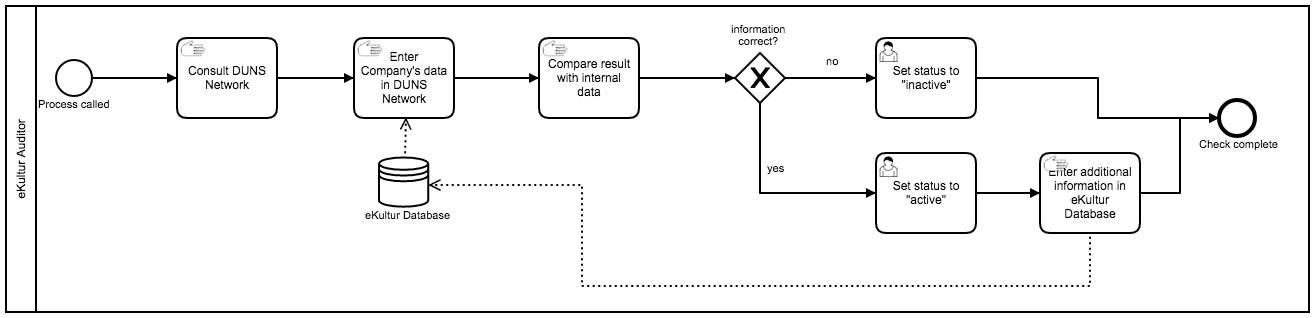
\includegraphics[scale=0.4]{../figures/chapter_casestudy/company_audit/BPMN_Check_DUNS.png} 
\caption{\textit{Check DUNS Number} process modeled in BPMN.}
\label{fig:duns_number_BPMN}
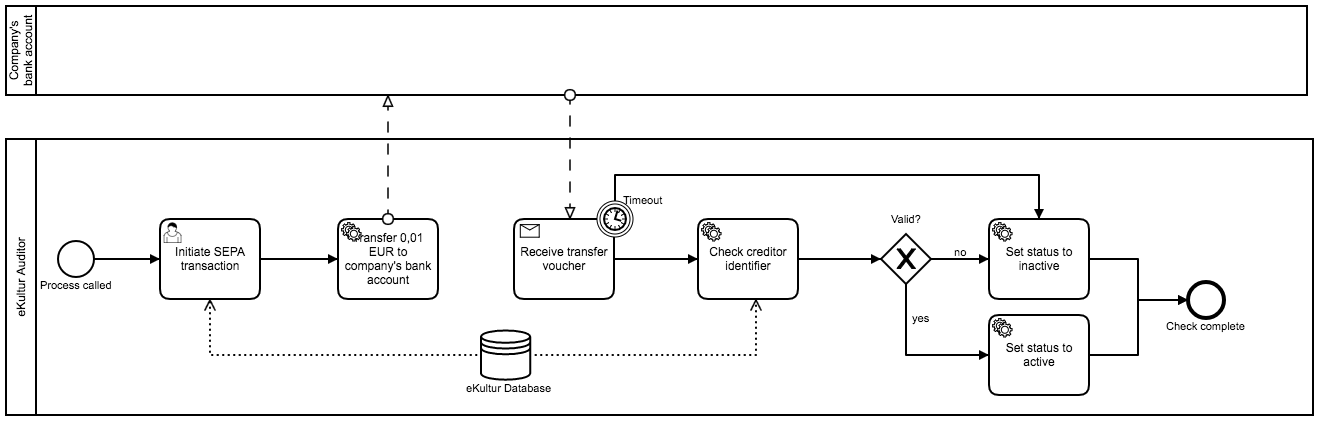
\includegraphics[scale=0.4]{../figures/chapter_casestudy/company_audit/BPMN_Check_Creditor_Identifier.png}  
\caption{\textit{Check Creditor Identifier} process modeled in BPMN.}
\label{fig:creditor_identifier_BPMN}
\end{sidewaysfigure}

\subsubsection{Check Creditor Identifier}
A Creditor Identifier is a number generated similar to a barcode. The number has a total length of 18 and is comprised of an ISO Country-code that identifies the country where the company's headquarter is located, followed by a checksum and a creditor business code indicating the commercial activity \footnote{taken from  Deutsche Bundesbank \url{https://www.bundesbank.de/} (Oct. 12, 2016)}.\\
The German Federal Bank, similar to DUNS and the Federal Gazette, do not offer any interface to validate a creditor identifier and assure the authenticity. Ideally, an interface to their database would initiate a comparison that outputs either a validated status or the opposite. In this case, the \textit{Check Creditor Identifier} process initiates a \ac{SEPA} transaction that returns a receipt including the company's creditor identifier. Similar to procedures known from major payment integrator platforms such as PayPal, the transaction assures on the one hand the company's bank account's authenticity and on the other hand the creditor identifier.\\
According to the process documentation, the workflow should be automated. A service handles the \ac{SEPA} transaction and waits for the transaction voucher that contains the creditor identifier. When received, the voucher is scanned for the creditor identifier, which is then compared with the one stored in the internal database. If the values match, the company's status is set to \textit{active}, otherwise to \textit{inactive}. \\
Concluding the process discovery for this sub-process, the objective is to automate the complete workflow, so the auditor has only to initiate the process. Apart from this step, all further tasks are intended to work without human intervention or run-time adjustment. The process is rigid, predefined and workflow-centric, paired with a strict control flow and simple decisions. For all sub-processes, the preceding process map is the one presented earlier in this section and represents a cluster. This leads to a small match with CMMN, as seen in Table \ref{tab:creditor_identifier}. However, the threshold of 80\% is exceeded for BPMN leading to a recommendation for this modeling language. Figure \ref{fig:creditor_identifier_BPMN} shows the model created with the BPMN notation. 

% Please add the following required packages to your document preamble:
% \usepackage{booktabs}
% \usepackage{graphicx}
\begin{table}[]
\centering
\resizebox{\textwidth}{!}{%
\begin{tabular}{@{}lllll@{}}
\toprule
Categories                   & Check Creditor Identifier matches   & BPMN Points & CMMN Points & DMN Points \\ \midrule
Documentation style          & Directives                          & 1           & 0           & 0          \\
Preceding process map        & Cluster                             & 0           & 1           & 0          \\
Characteristics of work      & routine, predictable                & 2           & 0           & 0          \\
Characteristics of process   & rigid, predefined, workflow-centric & 2           & 0           & 0          \\
Characteristics of decisions & Simple (either / or)                & 2           & 0           & 0          \\
Control flow                 & Definite control flow, required     & 1           & 0           & 0          \\
Intervention at run-time     & No                                  & 1           & 0           & 0          \\
Objective                    & Automated workflow execution        & 2           & 0           & 0          \\
Type of process              & Business process                    & 2           & 0           & 0          \\
Typical application          & Accounting                          & 1           & 0           & 0          \\ \midrule
\multicolumn{2}{l}{Percentage}                                     & 93,33       & 6,67        & 0          \\ \bottomrule
\end{tabular}%
}
\caption{Indicator application on the \textit{Check Creditor Identifier} process.}
\label{tab:creditor_identifier}
\end{table}

\subsubsection{Check Website}
A rather weak check of the company's authenticity is to examine their online presence. Both, touring theater production industry and their supplying industry still operate mainly without relying on online tools. For this reason, eKultur started the project to develop this offline industry into an online one, creating a portal where all the different participants of a workflow can cooperate. Currently few of the industry's members run a website or even advanced online technology. Therefore, the \textit{Check Website} process serves as an optional one supporting the auditor in case of arising uncertainty about the company's existence. \\
These circumstances lead to partly predefined processes and indefinite control flows. The auditor is intended to work in a knowledge-driven manner that requires him to decide what to do according to emerging circumstances. This is proved by the documentation and the way it describes the sub-process. In contrast to earlier examined sub-processes documented in a directive way, this one features a description of work instead of a strict plan. The process analysts refer to the auditor's discretion as the central part of the process with the goal to support his manual work. However, the process does not feature stateful decisions but rather simple ones. Overall, the process can be described as a review and represents a case instead of a business process, as Table \ref{tab:check_website} indicates. With an accordance of 86,67\%, the indicators recommend CMMN as a suitable language. Figure \ref{fig:check_website_CMMN} represents the resulting CMMN model according to the process documentation.

% Please add the following required packages to your document preamble:
% \usepackage{booktabs}
% \usepackage{graphicx}
\begin{table}[]
\centering
\resizebox{\textwidth}{!}{%
\begin{tabular}{@{}lllll@{}}
\toprule
Categories                   & Check Website matches & BPMN Points & CMMN Points & DMN Points \\ \midrule
Documentation style          & Description           & 0           & 1           & 0          \\
Preceding process map        & Cluster               & 0           & 1           & 0          \\
Characteristics of work      & Agile                 & 0           & 2           & 0          \\
Characteristics of process   & partly predefined     & 0           & 2           & 0          \\
Characteristics of decisions & Simple (either / or)  & 2           & 0           & 0          \\
Control flow                 & Indefinite            & 0           & 1           & 0          \\
Intervention at run-time     & Yes                   & 0           & 1           & 0          \\
Objective                    & Support Manual Work   & 0           & 2           & 0          \\
Type of process              & Case                  & 0           & 2           & 0          \\
Typical application          & Review                & 0           & 1           & 0          \\ \midrule
\multicolumn{2}{l}{Percentage}                       & 13,33       & 86,67       & 0          \\ \bottomrule
\end{tabular}%
}
\caption{Indicator application on the \textit{Check Website} process.}
\label{tab:check_website}
\end{table}

\begin{sidewaysfigure}
\centering 
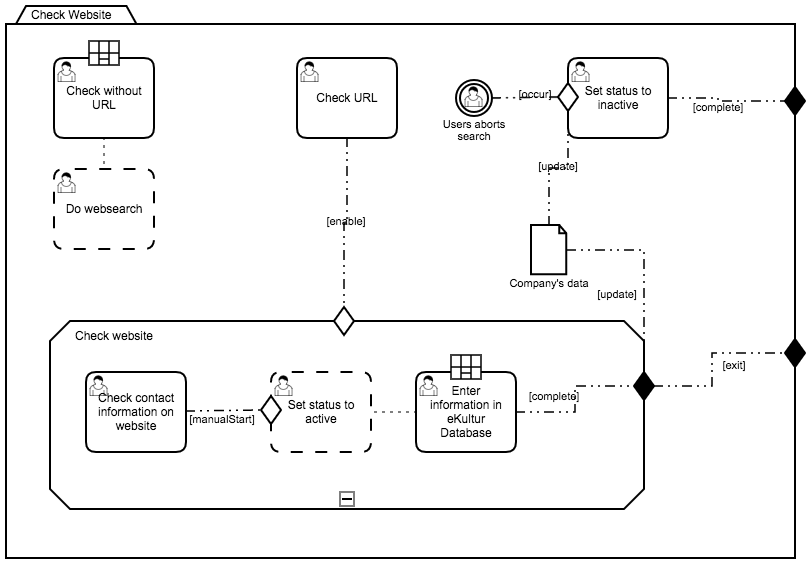
\includegraphics[width=0.9\textwidth]{../figures/chapter_casestudy/company_audit/CMMN_Check_Website.png} 
\caption{\textit{Check Website} process modeled in CMMN.}
\label{fig:check_website_CMMN}
\end{sidewaysfigure}

\subsubsection{Check Current Media}
Another research task is the check for current media activities. If a company is an active market participant, current media could report about their activities. Especially theater production companies are interested in press coverage about their productions on stage or awards they might receive. Consequently, the auditor is able to get an idea of the current state of the company and perform different checks such as personal contact, if necessary. \\
A similarity between the \textit{Check Website} and \textit{Check Current Media} process can be observed and the indicators confirm this hypothesis. Table \ref{tab:check_current_media} summarizes the characteristics of the process that were found during process discovery. \\
The concept is derived from the \textit{Check Website} process, explaining why the documentation for this process is less detailed compared to the mentioned original. Thus, the suitable language is also CMMN as the indicators identify. Both processes support the auditor's investigation if the company is trustworthy or not. Figure \ref{fig:check_current_media_CMMN} displays the CMMN model.

% Please add the following required packages to your document preamble:
% \usepackage{booktabs}
% \usepackage{graphicx}
\begin{table}[]
\centering
\resizebox{\textwidth}{!}{%
\begin{tabular}{@{}lllll@{}}
\toprule
Categories                   & Check Current Media matches & BPMN Points & CMMN Points & DMN Points \\ \midrule
Documentation style          & Description                 & 0           & 1           & 0          \\
Preceding process map        & Cluster                     & 0           & 1           & 0          \\
Characteristics of work      & Agile                       & 0           & 2           & 0          \\
Characteristics of process   & partly predefined           & 0           & 2           &            \\
Characteristics of decisions & Simple (either / or)        & 2           & 0           & 0          \\
Control flow                 & Indefinite                  & 0           & 1           & 0          \\
Intervention at run-time     & Yes                         & 0           & 1           & 0          \\
Objective                    & Support Manual Work         & 0           & 2           & 0          \\
Type of process              & Case                        & 0           & 2           & 0          \\
Typical application          & Review                      & 0           & 1           & 0          \\ \midrule
\multicolumn{2}{l}{Percentage}                             & 13,33       & 86,67       & 0          \\ \bottomrule
\end{tabular}%
}
\caption{Indicator application on the \textit{Check Current Media} process.}
\label{tab:check_current_media}
\end{table}

\begin{sidewaysfigure}
\centering 
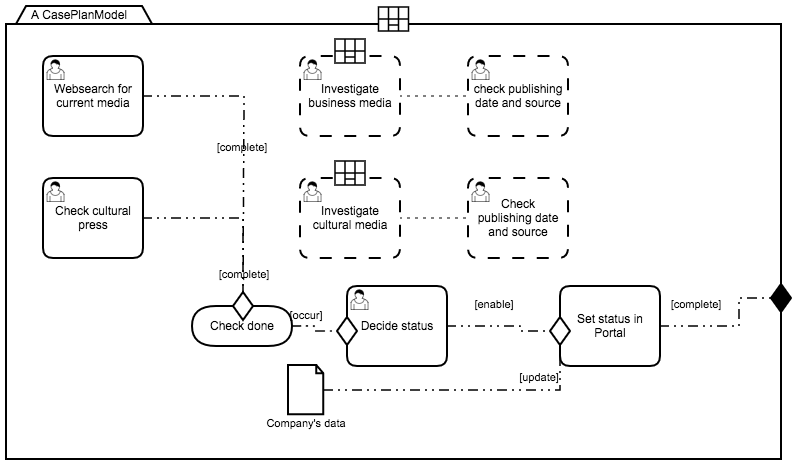
\includegraphics[width=0.9\textwidth]{../figures/chapter_casestudy/company_audit/CMMN_Check-Media.png} 
\caption{\textit{Check Current Media} process modeled in CMMN.}
\label{fig:check_current_media_CMMN}
\end{sidewaysfigure}

\subsubsection{Personal Contact}
Another option to check the authenticity of a company is making personal contact. The theater production industry in Germany is a rather small one, consequently a large amount of participants cooperate or at least keep in touch during an accounting year. For this reason, the auditor's knowledge about a certain company should be captured in this series of checks. \\
The eKulturPortal implements the concept of \textit{Crowdsourcing}. Similar to Wikipedia, users are intended and motivated to accomplish certain tasks such as reporting deprecated addresses or, in this case, bail for a company's authenticity. The auditor may set the status to active, if a certain threshold is reached (e.g. five references by already checked members). \\
At the current stage of development, the crowdsourcing aspect is not ready for implementation, therefore we can only provide and interface in this sub-process. Clearly, this process cannot be modeled in BPMN or DMN since the focus is on the auditor's choice on how to execute this check. Apart from the interface, the whole process features agile work and a knowledge-centric approach (see Table \ref{tab:personal_contact}). Furthermore, the decisions need to be stateful, as the completion of checks is followed by writing a report and eventually exiting a case. \\
Especially the latter task resembles a typical reviewing process leading to the \textit{Review} term in the \textit{Typical Application} category.\\
Overall, this process achieves a 100\% match with the CMMN indicators. The interface to the references process, however, was not covered by this indicator analysis. Generally, a \textit{call}-task should not be covered by the indicator analysis, since the logic is encapsulated in the process called by this task. The resulting model is provided in Figure \ref{fig:personal_contact_CMMN}. 

% Please add the following required packages to your document preamble:
% \usepackage{booktabs}
% \usepackage{graphicx}
% \usepackage[normalem]{ulem}
% \useunder{\uline}{\ul}{}
\begin{table}[]
\centering
\resizebox{\textwidth}{!}{%
\begin{tabular}{@{}lllll@{}}
\toprule
Categories                   & Personal Contact matches             & BPMN Points & CMMN Points & DMN Points \\ \midrule
Documentation style          & Description                          & 0           & 1           & 0          \\
Preceding process map        & Cluster                              & 0           & 1           & 0          \\
Characteristics of work      & Agile, emerging                      & 0           & 2           & 0          \\
Characteristics of process   & partly predefined, knowledge-centric & 0           & 2           & 0          \\
Characteristics of decisions & Stateful                             & 0           & 2           & 0          \\
Control flow                 & Indefinite                           & 0           & 1           & 0          \\
Intervention at run-time     & yes                                  & 0           & 1           & 0          \\
Objective                    & Support Manual Work                  & 0           & 2           & 0          \\
Type of process              & Case                                 & 0           & 2           & 0          \\
Typical application          & Review                             & 0           & 1           & 0          \\ \midrule
\multicolumn{2}{l}{Percentage}                                      & 0           & 100         & 0          \\ \bottomrule
\end{tabular}%
}
\caption{Indicator application on the \textit{Personal Contact} process.}
\label{tab:personal_contact}
\end{table}

\begin{sidewaysfigure}
\centering 
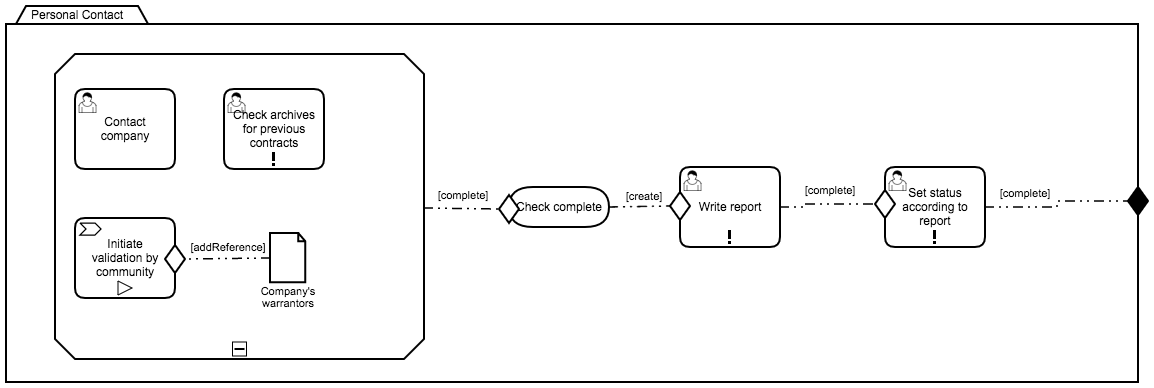
\includegraphics[width=0.9\textwidth]{../figures/chapter_casestudy/company_audit/CMMN_Personal_Contact.png} 
\caption{\textit{Personal Contact} process modeled in CMMN.}
\label{fig:personal_contact_CMMN}
\end{sidewaysfigure}

\subsection{Combining the sub-processes}
In the previous subsections we analyzed the sub-processes and applied the indicators on them to find a suitable modeling notation. There is still one missing piece to complete the process modeling: the orchestrating superstructure. In fact, this superstructure is another process where we can apply the indicators to find the suitable notation. \\
First of all, a look at the process documentation indicates that this process does not require a strict control flow. Emphasized by the process map in Figure \ref{fig:company_audit_PM}, the structure resembles more of a cluster instead of a workflow. The process documentation focuses on the auditor's discretion on how and when to execute the steps. To be precise, the documentation encapsulates the logic of the checks in several bullet points but does not explain, when to execute a certain task and in what sequence. \\
During the analysis of the sub-processes we saw that some of the checks are used for optional research, whereas some of them check hard facts. This leads to a prioritization of checks and a sequence we can capture in the resulting model. For this reason, DMN is again not a suitable solution due missing structural elements.\\
Another indicator that can be determined is the decision structure. Basically, the checks need to be done and the auditor needs to set an internal status that either is \textit{valid} or \textit{invalid} afterwards. On the way to this simple decision, each performed check has a transition from \textit{enabled} to \textit{active} and eventually to \textit{completed} or \textit{terminated}. In fact, these states are the decisions the auditor has to make during the process. He has to either complete the check or abort it. As a result, the decisions are stateful and indicate DMN in this case. \\
Conclusively, the process resembles a review, is a case and should be modeled in CMMN. Table \ref{tab:company_audit_CMMN} indicates a 100\% match with the CMMN indicators. 

%-------------------------------------------------------------------------
% Please add the following required packages to your document preamble:
% \usepackage{booktabs}
% \usepackage{graphicx}
% \usepackage[normalem]{ulem}
% \useunder{\uline}{\ul}{}
\begin{table}[]
\centering
\resizebox{\textwidth}{!}{%
\begin{tabular}{@{}lllll@{}}
\toprule
Categories                   & Company Audit matches       & BPMN Points & CMMN Points & DMN Points \\ \midrule
Documentation style          & Description                 & 0           & 1           & 0          \\
Preceding process map        & Cluster                     & 0           & 1           & 0          \\
Characteristics of work      & agile, partly automatable   & 0           & 2           & 0          \\
Characteristics of process   & partly predefined, adaptive & 0           & 2           & 0          \\
Characteristics of decisions & Stateful                    & 0           & 2           & 0          \\
Control flow                 & Indefinite                  & 0           & 1           & 0          \\
Intervention at run-time     & Yes                         & 0           & 1           & 0          \\
Objective                    & Support manual work         & 0           & 2           & 0          \\
Type of process              & Case                        & 0           & 2           & 0          \\
Typical application          & Review                      & 0           & 1           & 0          \\ \midrule
\multicolumn{2}{l}{Percentage}                             & 0           & 100         & 0          \\ \bottomrule
\end{tabular}%
}
\caption{Indicator application on the \textit{Company audit} super-process.}
\label{tab:company_audit_CMMN}
\end{table}

%-------------------------------------------------------------------------

\begin{sidewaysfigure}
\centering 
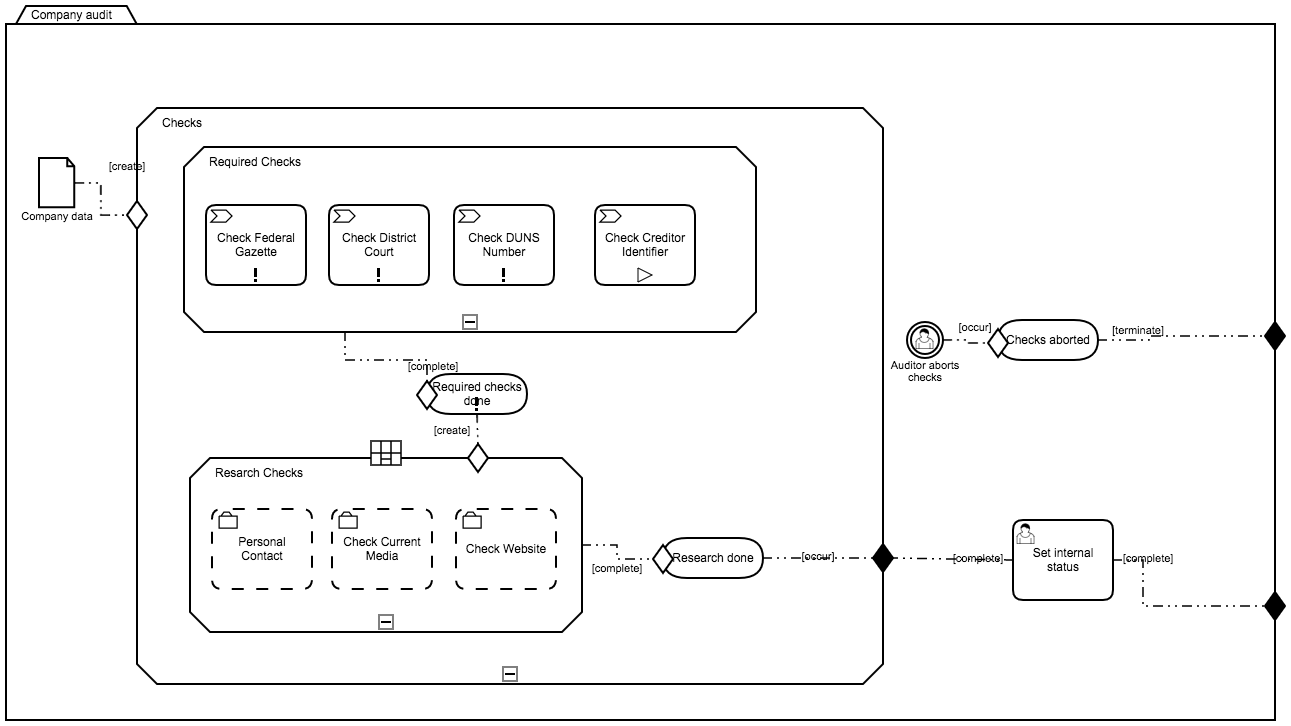
\includegraphics[width=\textwidth]{../figures/chapter_casestudy/company_audit/CMMN_Company_Audit.png} 
\caption{The \textit{Company Audit} process modeled in CMMN.}
\label{fig:company_audit}
\end{sidewaysfigure}
%-------------------------------------------------------------------------

In Chapter \ref{chapter:combination}, various possible ways of how to combine modeling languages were presented along with the corresponding interfaces. The \textit{Company Audit} process model represents a way to apply these findings on a real use case. Figure \ref{fig:company_audit} shows the process modeled in CMMN. Each sub-process is notated as an interface to the corresponding logical unit that is called upon activation. Stages separate the required from the research ones and put them at the beginning of the process. \\
There are several notable objects included in the model that are not mentioned in the process discovery, though useful during execution. The process starts by opening the CaseFileItem that creates the Stage \textit{Checks}. This assures that each update of the CaseFileItem, ergo loading a different file from the database, generates new checks. \\
Next, there are Milestones implemented that are not mentioned in the process documentation. Milestones are elements, according to \cite{CMMNspec2014}, that support monitoring the progress of each case. Consequently, the platform will able to send the company a status update about the audition during execution. \\
As a side-effect, the process is also more structured. After reaching the first Milestone, the research stage is instantiated and its execution can be planned. This assures, that all the necessary checks are completed before the investigation of current media or websites commences. The exact execution, however, is still to the auditors discretion along with planning the further investigation or even aborting the audit, if necessary. \\
In the end, the exit of a case can be achieved by completing the \textit{Checks} stage, with or without any further investigation as these tasks are discretionary ones. In contrast to the required checks, the research ones do not feature an exclamation mark indicating the \textit{Required Rule}. If so, these tasks need to be executed and a completion of the stage can only be achieved after completing each required task. The \textit{Research checks} stage does not feature any elements with \textit{Required Rule} set to \texttt{true}. \\

\section{Create New Venue}

\begin{figure}[!ht]
\centering
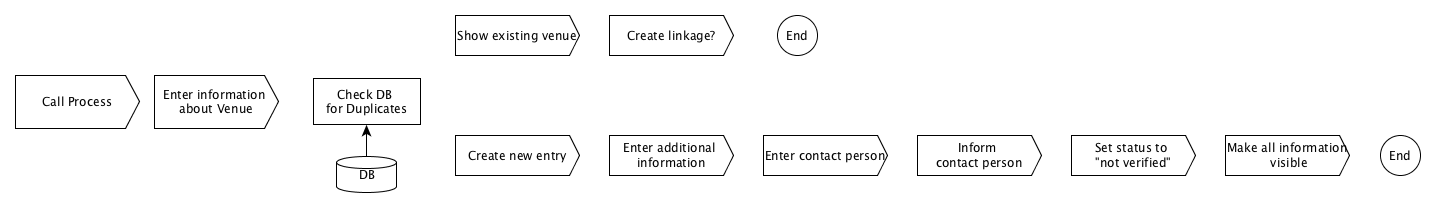
\includegraphics[width=\textwidth]{../figures/chapter_casestudy/Create_New_Venue_PM.png} 
\caption{\textit{Create New Venue} process map resembling a flow chart.}
\label{fig:create_new_venue_PM}
\end{figure}

An essential part of theater production is bringing a play on stage. Of course, this is the reason plays are produced for and the highlight of each production. To assure a trouble-free performance, information about the venue and especially the stage is important. The current workflow requires either calling the venue's contact person or relying on information that is already gathered. However, knowledge about the stages and venues is, seen from the whole industry aspect, implicit. Thus, there is an opportunity for the platform to aggregate this implicit knowledge and publish it. For this reason, the portal features entities called \textit{Venues}. \\
The eKulturPortal features two sorts of venues: ones that are administered by \textit{active} and \textit{validated} companies, thus the venues are also active and validated, allowing interested users to book them eventually. The other ones are not yet \textit{validated} due to a missing administrating company or one that is also not yet validated. Consequently, these venues are entities the user cannot book. The following process deals with venues that are not yet validated or whose company is not available in the system yet. \enlargethispage{1\baselineskip} \newpage Appendix B provides the process discovery output, which serves as basement for the following analysis. \\
The \textit{Create New Venue} process is a rather small process that features only a few steps. A process map corresponding to the process documentation is provided in Figure \ref{fig:create_new_venue_PM}, resembling a flow chart. The purpose of this process map was to structure the process and identify major steps and their sequence. Furthermore, the process map indicates a definite control flow, although the process presumably features some manual parts such as entering the venue's information. \\
Having a look at the structure of the process documentation we notice an orchestration that can also be seen in the process map. Consequently, we can assign a BPMN point for a \textit{directing process documentation}. The captured workflow comprises routine aspects along with a completely predefined output. The process is intended to be workflow-centric and rigid with the necessity of run-time intervention. In contrast to CMMN cases, the workflow execution is intended to proceed without any adaptions. In case of emerging failures, the user is guided by the interface to either an earlier step of the process or he is able to abort and restart it. These are the two adjustments the process is intended to allow. This part is not explicitly mentioned in the process documentation, but can be derived from the overall impression the documentation makes.\\
As this is not a real business process, we cannot assign this point to the BPMN indicators and need to leave this part. In fact, each process mentioned in this thesis cannot be described as real \textit{business processes}, since the portal's business part is neither designed nor implemented yet. Each process is part of the \textit{address data} milestone, ultimately allowing the users to exchange and administrate their address data and corresponding entities such as companies or venues.\\
Since the process does not feature any complex data handling apart from storing the entered information in a database, we can set the decisions to \textit{simple}. Different from \textit{stateful} ones, simple decisions do not allow status handling and thus are sufficient for this process. \\
Concluding the analysis, Table \ref{tab:create_new_venue} shows the results and recommends to model the process in BPMN. Due to the repeatability of the process, the \textit{Typical Application} was set to \textit{Assembly-line work}. The users are intended to create venue-entities in the system and fill the portal with information about available stages.\\
The resulting model is shown in Figure \ref{fig:create_new_venue_BPMN}, capturing the steps it takes to create a new venue along with the approval that is necessary to show all information about it. Due to German Data Protection Act, all information about the venue and the contact person cannot be provided without the person's permission. \\
Consequently, a message is sent to the contact person asking for permission to publish the data. If approved, the entity is published without any restrictions. Otherwise, the information is published with limited information.\\
For this process, the indicators recommended BPMN and it turned out this notation was suitable for modeling the process. The characteristics described in Table \ref{tab:create_new_venue} are represented in the model, such as routine aspects, the automation-objective and the definite control flow along with a rigid structure. 


% Please add the following required packages to your document preamble:
% \usepackage{booktabs}
% \usepackage{graphicx}
\begin{table}[]
\centering
\resizebox{\textwidth}{!}{%
\begin{tabular}{@{}lllll@{}}
\toprule
Categories                   & Create New Venue matches & BPMN Points & CMMN Points & DMN Points \\ \midrule
Documentation style          & Directives               & 1           & 0           & 0          \\
Preceding process map        & Flowchart                & 1           & 0           & 0          \\
Characteristics of work      & routine, predictable     & 2           & 0           & 0          \\
Characteristics of process   & rigid, workflow-centric  & 2           & 0           & 0          \\
Characteristics of decisions & Simple                   & 2           & 0           & 0          \\
Control flow                 & Definite                 & 1           & 0           & 0          \\
Intervention at run-time     & No                       & 1           & 0           & 0          \\
Objective                    & Automation               & 2           & 0           & 0          \\
Type of process              & -                        & 0           & 0           & 0          \\
Typical application          & Assembly-line work       & 1           & 0           & 0          \\ \midrule
\multicolumn{2}{l}{Percentage}                          & 86,67       & 0           & 0          \\ \bottomrule
\end{tabular}%
}
\caption{Indicator application on the \textit{Create New Venue} process.}
\label{tab:create_new_venue}
\end{table}

\begin{sidewaysfigure}[!h]
\centering 
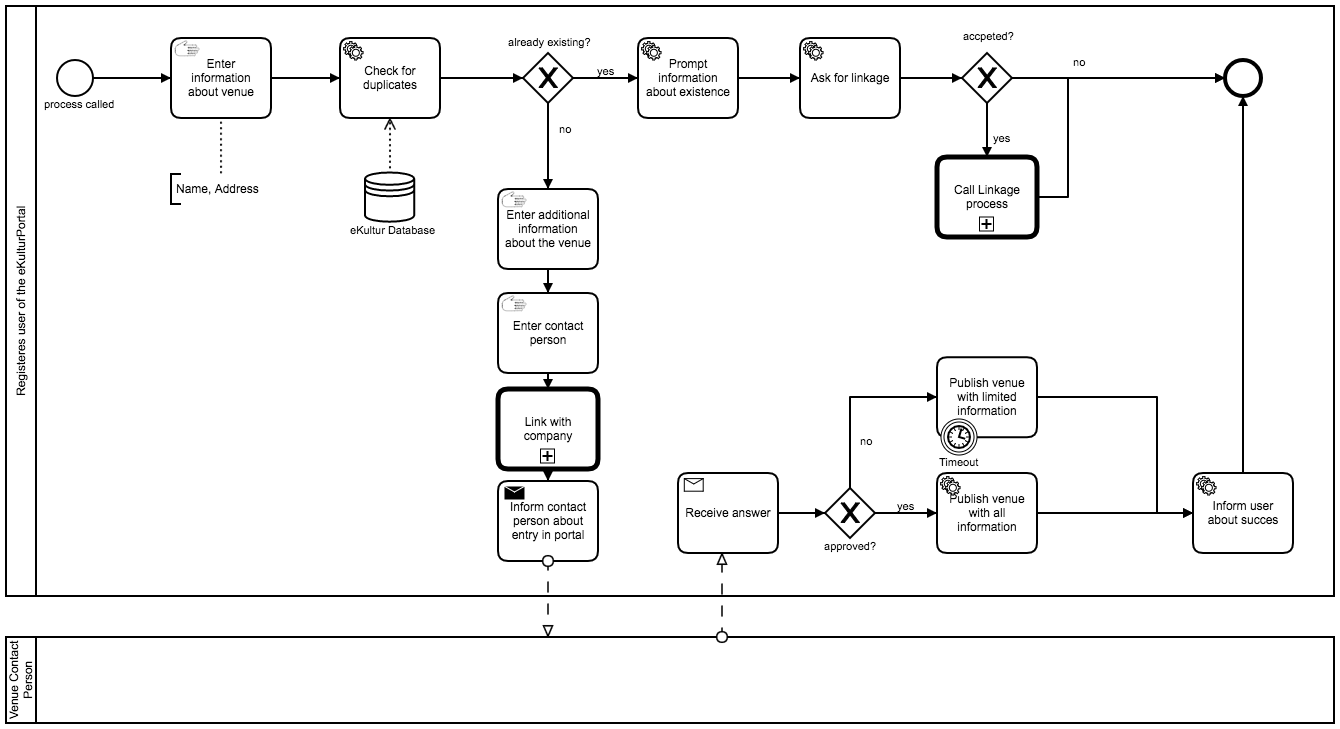
\includegraphics[width=\textwidth]{../figures/chapter_casestudy/BPMN_Create_Venue.png} 
\caption{The \textit{Create New Venue} process modeled in BPMN according to the indicators in Table \ref{tab:create_new_venue} and the process documentation in Appendix B.}
\label{fig:create_new_venue_BPMN}
\end{sidewaysfigure} 

\section{Create New Company} 
In a previous section, the \textit{Company audit} process was presented along with an analysis and recommendation for a suitable notation. The foundation for auditing companies are existing entries in the eKultur database. When the portal is being published initially and first users are invited to work with it, creating companies will be one of the very first steps that need to be done. Creating new entries has several requirements such as authenticity and singularity, combined with information density and the ability to link them with either users or different companies. The latter one  also defines business relationships and is intended to generate contracts completely automatically. After reaching the first milestone, however, the main functionality users are able to use will be administering and linking companies, as well as users and eventually clustered organizations.\\
Appendix C features the process documentation for the \textit{Create New Company} process and describes in a directive way how the process should be executed.\newpage eKultur expects a user base of more than one hundred companies after two years, due to the small amounts of business participating in the industry. eKultur itself only has a few employees, which holds true for ever associated partner of the project and the competitors apart from few larger ones. As a consequence, the process to create new company entries will be executed approximately one hundred times and therefore is a routine task of the portal.\\
Each company entry is comprised of information that uniquely identifies it. Among others, name and address as well as the creditor identifier and the commercial registry number identify the company both in the system when it comes to duplicates, and during the \textit{Company audit} process, when the company is being checked by the eKultur auditors. Thus, the process needs to be rigid without allowing the user to adapt any execution sequence during run-time. The entries need to be created exactly as intended to assure a working system. \\
Therefore, the process is completely predefined and workflow-centric. This can be derived from the directive style of the process documentation. There is no room for any interpretation or planning left. However, for this process a process map was not created, making it more difficult to model the process afterwards. A rough impression about the process orchestration makes it easier for the analysts to create the resulting model with the recommended modeling language after the analysis phase. \\
Comparing the process with a case or a business process is neither possible, since the process does not incorporate any business logic. Comparing it with a typical application, it resembles the assembly-line workflow, due to major routine aspects of the process. Users are intended to create company entries during the initial phase as much as possible, very similar to an assembly-line that creates a large amount of the very same product without much deviation. \\
Table \ref{tab:create_new_company} concludes the findings from the process discovery documented in Appendix C. A threshold of 80\% is reached, therefore BPMN is recommended by the indicators. The resulting model can be found in Figure \ref{fig:create_new_company_BPMN}, featuring the characteristics the process discovery showed and Table \ref{tab:create_new_company} indicated: The process has a rigid structure, combined with simple decisions and a vast amount of automated tasks, such as the \textit{Check for duplicates} task. A definite control flow suits best for this routine process and assures the exact execution, resulting in predictable results only deviating in specific information the objects contain. Neither CMMN (supporting manual work), nor DMN (processing data) would be suitable in this case. 
%--------------------------------------------------------------------------------------------------------------
% Please add the following required packages to your document preamble:
% \usepackage{booktabs}
% \usepackage{graphicx}
\begin{table}[]
\centering
\resizebox{\textwidth}{!}{%
\begin{tabular}{@{}lllll@{}}
\toprule
Categories                   & Create New Company matches          & BPMN Points & CMMN Points & DMN Points \\ \midrule
Documentation style          & Directives                          & 1           & 0           & 0          \\
Preceding process map        & -                                   & 0           & 0           & 0          \\
Characteristics of work      & routine, predictable, automatable   & 2           & 0           & 0          \\
Characteristics of process   & rigid, predefined, workflow-centric & 2           & 0           & 0          \\
Characteristics of decisions & Simple                              & 2           & 0           & 0          \\
Control flow                 & Definite                            & 1           & 0           & 0          \\
Intervention at run-time     & No                                  & 1           & 0           & 0          \\
Objective                    & Automation                          & 2           & 0           & 0          \\
Type of process              & -                                   & 0           & 0           & 0          \\
Typical application          & Assembly-line work                  & 1           & 0           & 0          \\ \midrule
\multicolumn{2}{l}{Percentage}                                     & 80          & 0           & 0          \\ \bottomrule
\end{tabular}%
}
\caption{Indicator application on the \textit{Create New Company} process.}
\label{tab:create_new_company}
\end{table}

%--------------------------------------------------------------------------------------------------------------

\begin{sidewaysfigure}
\centering
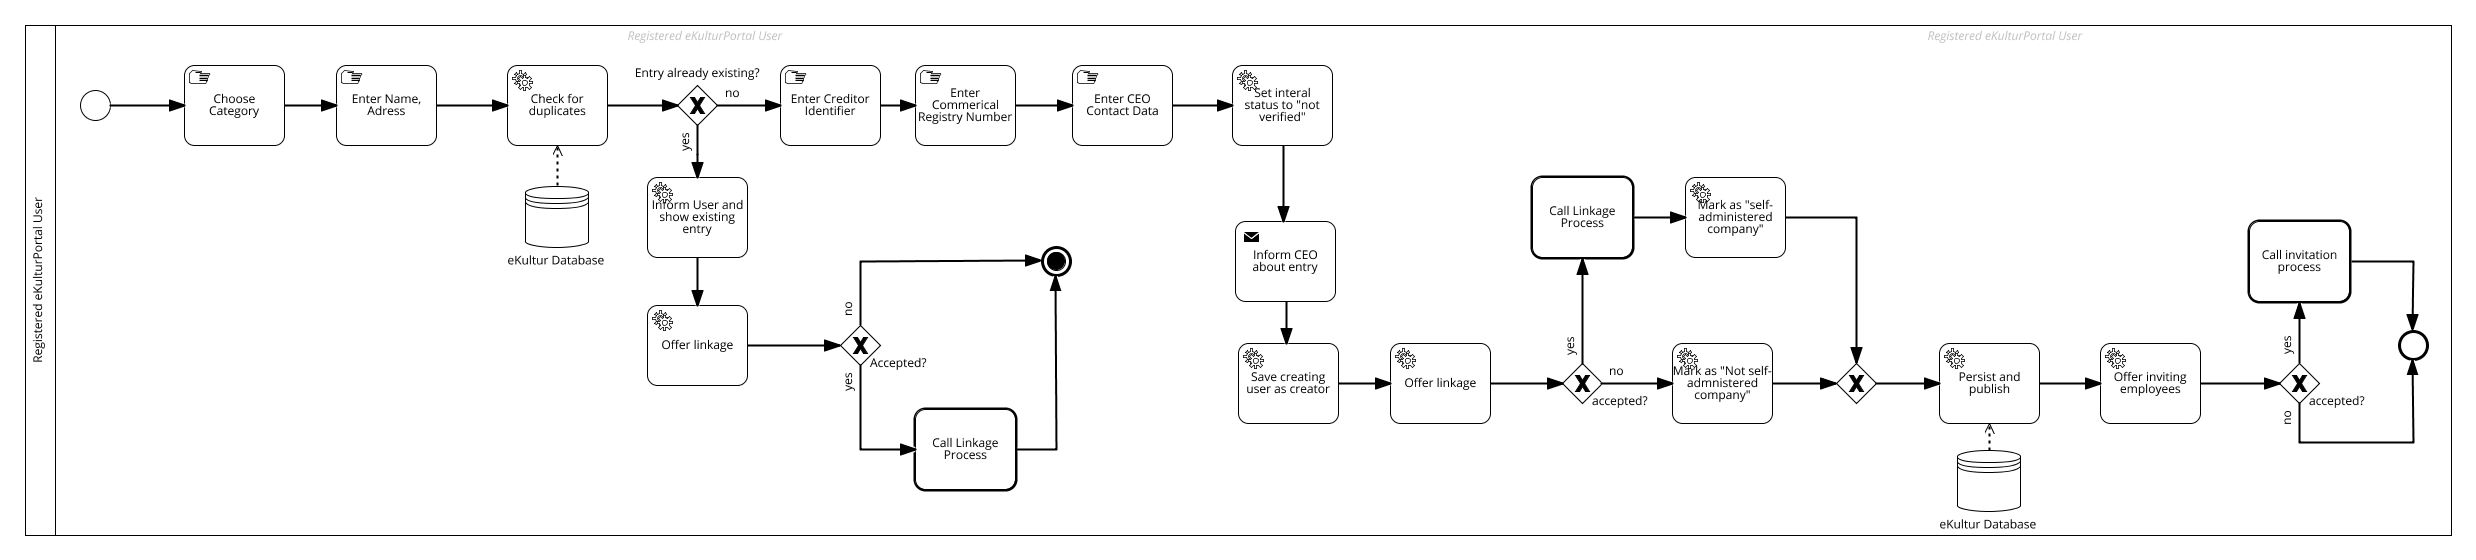
\includegraphics[width=\textwidth]{../figures/chapter_casestudy/Create_New_Company_BPMN.png}
\caption{The \textit{Create New Company} process modeled in BPMN according to the indicators in Table \ref{tab:create_new_company} and the process documentation in Appendix C}
\label{fig:create_new_company_BPMN}
\end{sidewaysfigure}

%--------------------------------------------------------------------------------------------------------------

\section{Summary}
In the preceding sections, the practical application of the indicators on process documentation taken from the eKulturPortal project was presented. At first, a methodology on how to achieve a recommendation with the aid of a weighting system was introduced. On this basis, the recommendation could be calculated by averaging the weights. \\
Conclusively, the majority of these processes resulted in BPMN models. BPMN is and has been a very popular and broad modeling notation for processes. However, certain processes are better modeled in CMMN due to their agile characteristics and the flexible way of execution. Additional run-time adjustments, as well as a roughly predefined set of tasks complete these processes. What we haven't seen in this chapter was the application of indicators resulting in a recommendation for DMN. This is due to the complementary aspect of the DMN notation, making it easy to incorporate data processing but impractical for different use cases. As the preceding processes did not deal with actual data processing, the DMN notation could not be recommended for any of them. \\
The current state of the eKulturPortal only allows us to model processes dealing with address management and the handling of entities, but not with actual business processes which might lead to a recommendation for the DMN notation. This could be part of a future work and will be discussed in detail in the next chapter, along with positive and negative aspects of the application. 